\documentclass{beamer}

% Theme choice:
\usetheme{CambridgeUS}

%Packages
\usepackage[backend=biber,hyperref=true,doi=false,url=false,isbn=false, uniquename=false, uniquelist=false, style = authoryear-comp]{biblatex}
%https://www.overleaf.com/learn/latex/Biblatex_citation_styles
\addbibresource{synthVolForecast.bib}

%\usepackage{bibentry}

\usepackage{graphicx}
\usepackage{amsmath}
\usepackage{amsfonts}
\usepackage{amsthm}
\usepackage[export]{adjustbox}
\usepackage{amssymb}
\usepackage[useregional]{datetime2}
\usepackage{verbatim}
\usepackage{mathtools}% http://ctan.org/pkg/mathtools
\usepackage{mathrsfs}


\usepackage{amscd}
\usepackage{url}
% \usepackage[table,xcdraw,usenames]{xcolor}
% \usepackage[usenames]{color}

\usepackage{subcaption}
% \usepackage{enumitem}
% \usepackage{authblk}
% \usepackage{bm}
% \usepackage{pdfpages}

\usepackage{hyperref}
\usepackage{caption}
\usepackage{float}
%\usepackage[caption = false]{subfig}
\usepackage{tikz}
\usepackage{multirow}
\usepackage[linesnumbered, ruled,vlined]{algorithm2e}
\usepackage{pdflscape}
\usepackage{etoolbox}

%\AtBeginEnvironment{align}{\setcounter{equation}{0}} % https://tex.stackexchange.com/questions/349247/how-do-i-reset-the-counter-in-align

% function definition
\newcommand{\ret}{\textbf{r}}
\newcommand{\y}{\textbf{y}}
\newcommand{\w}{\textbf{w}}
\newcommand{\x}{\textbf{x}}
\newcommand{\dbf}{\textbf{d}}
\newcommand{\X}{\textbf{X}}
\newcommand{\Y}{\textbf{Y}}
% \newcommand{\L}{\textbf{L}}
\newcommand{\Hist}{\mathcal{H}}
\newcommand{\Prob}{\mathbb{P}}
\def\mbf#1{\mathbf{#1}} % bold but not italic
\def\ind#1{\mathrm{1}(#1)} % indicator function
\newcommand{\simiid}{\stackrel{iid}{\sim}} %[] IID
\def\where{\text{ where }} % where
\newcommand{\indep}{\perp \!\!\! \perp } % independent symbols
\def\cov#1#2{\mathrm{Cov}(#1, #2)} % covariance
\def\mrm#1{\mathrm{#1}} % remove math
\newcommand{\reals}{\mathbb{R}} % Real number symbol
\def\t#1{\tilde{#1}} % tilde
\def\normal#1#2{\mathcal{N}(#1,#2)} % normal
\def\mbi#1{\boldsymbol{#1}} % Bold and italic (math bold italic)
\def\v#1{\mbi{#1}} % Vector notation
\def\mc#1{\mathcal{#1}} % mathical
\DeclareMathOperator*{\argmax}{arg\,max} % arg max
\DeclareMathOperator*{\argmin}{arg\,min} % arg min
\def\E{\mathbb{E}} % Expectation symbol
\def\mc#1{\mathcal{#1}}
\def\var#1{\mathrm{Var}(#1)} % Variance symbol
\def\checkmark{\tikz\fill[scale=0.4](0,.35) -- (.25,0) -- (1,.7) -- (.25,.15) -- cycle;} % checkmark
\newcommand\red[1]{{\color{red}#1}}
\def\bs#1{\boldsymbol{#1}}
\def\P{\mathbb{P}}
\def\var{\mathbf{Var}}
\def\naturals{\mathbb{N}}
\def\cp{\overset{p}{\to}}
\def\clt{\overset{\mathcal{L}^2}{\to}}

\setcounter{tocdepth}{4}
\setcounter{secnumdepth}{4}

\newcommand{\ceil}[1]{\lceil #1 \rceil}
\newcommand{\norm}[1]{\left\lVert#1\right\rVert} % A norm with 1 argument
\DeclareMathOperator{\Var}{Var} % Variance symbol

\newtheorem{cor}{Corollary}
\newtheorem{lem}{Lemma}
\newtheorem{thm}{Theorem}
\newtheorem{defn}{Definition}
\newtheorem{prop}{Proposition}
\theoremstyle{definition}
\newtheorem{remark}{Remark}
\hypersetup{
  linkcolor  = blue,
  citecolor  = blue,
  urlcolor   = blue,
  colorlinks = true,
} % color setup

% % \makeatletter
% % \setbeamertemplate{footline}
% % {
% %     \leavevmode%
% %     \hbox{%
% %         \begin{beamercolorbox}[wd=.333333\paperwidth,ht=2.25ex,dp=1ex,center]{author in head/foot}%
% %             \usebeamerfont{author in head/foot}\insertshortauthor
% %         \end{beamercolorbox}%
% %         \begin{beamercolorbox}[wd=.333333\paperwidth,ht=2.25ex,dp=1ex,center]{title in head/foot}%
% %             \usebeamerfont{title in head/foot}\insertshorttitle
% %         \end{beamercolorbox}%
% %         \begin{beamercolorbox}[wd=.333333\paperwidth,ht=2.25ex,dp=1ex,right]{date in head/foot}%
% %             \usebeamerfont{date in head/foot}\insertshortdate{}\hspace*{2em}
% %             \insertframenumber{} / \inserttotalframenumber\hspace*{2ex}
% %         \end{beamercolorbox}}%
% %         \vskip0pt%
% %     }
% %     \makeatother

\title{Synthetic Volatility Forecasting and Other Aggregation Techniques for Time Series Forecasting}
\subtitle{Preliminary Exam}
\author{David Lundquist\thanks{davidl11@ilinois.edu}}
\date{\today}

\begin{document}

\part{one}
%% title frame
\begin{frame}
\titlepage
\end{frame}

\section{Introduction}

\begin{frame}
\frametitle{A seemingly unprecedented event might make one ask}
\begin{enumerate}
    \item What does it resemble from the past?
    \item What past events are most relevant?
    \item Can we incorporate past events in a systematic, principled manner?
\end{enumerate}
\end{frame}

\begin{frame}
    \frametitle{When would we ever have to do this?}

    \begin{itemize}
        \item Event-driven investing strategies (unscheduled news shock)
        \item Pairs trading strategies
        \item Structural shock to macroeconomic conditions (scheduled news possibly pre-empted by news shock)
        \item Biomedical panel data subject to exogenous shock or interference
    \end{itemize}
\end{frame}


\begin{frame}

    \begin{example}[Weekend of March 6th - 8th, 2020]
        \href{https://www.governor.ny.gov/news/novel-coronavirus-briefing-governor-cuomo-declares-state-emergency-contain-spread-virus}{
\includegraphics[scale=.3]{NYS_state.png}}

        \href{https://www.cnbc.com/2020/03/08/opec-deal-collapse-sparks-price-war-20-oil-in-2020-is-coming.html}{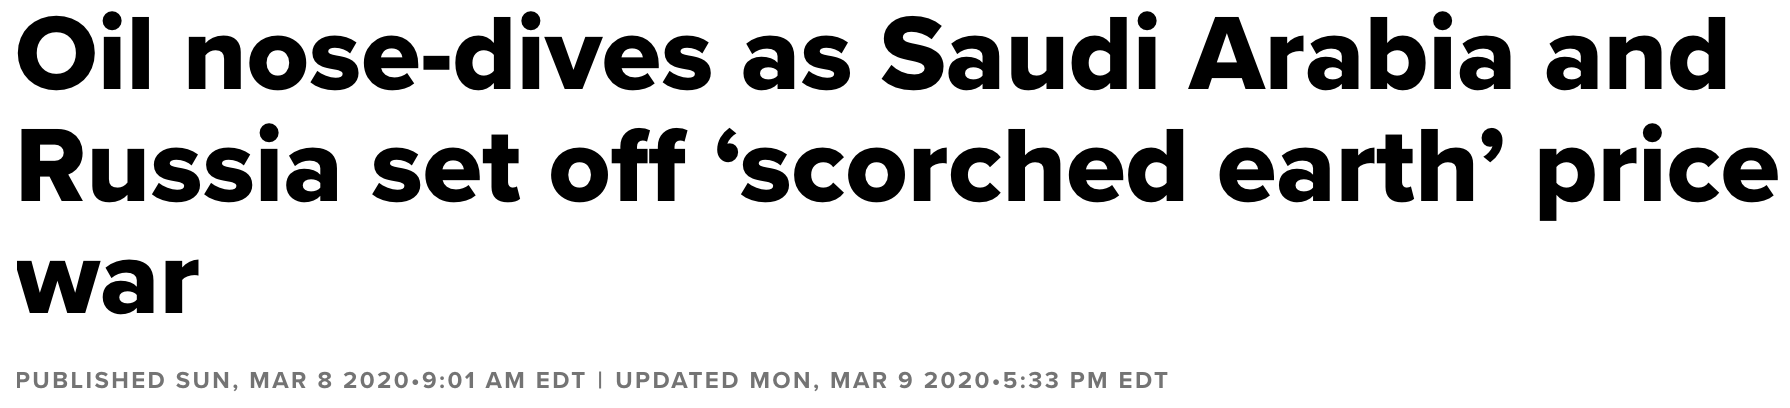
\includegraphics[scale=.3]{cnn.png}}

        \href{https://www.cnn.com/2020/03/08/investing/oil-prices-crash-opec-russia-saudi-arabia/index.html}{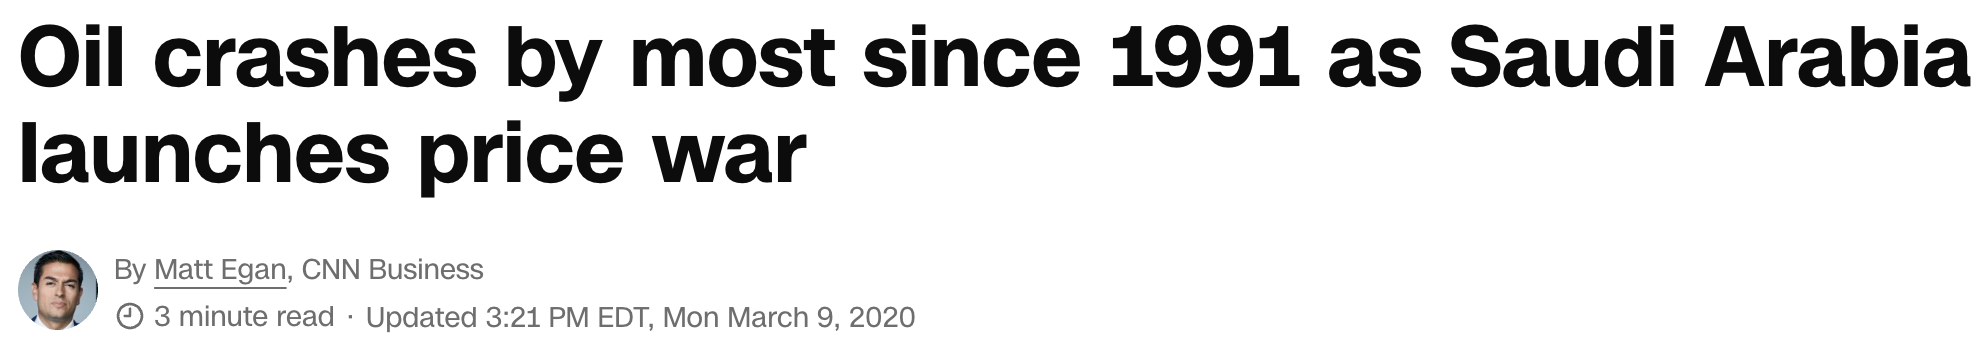
\includegraphics[scale=.3]{cnbc.png}}
        \end{example}


 
\end{frame}

\begin{frame}
\frametitle{Punchline of the paper}

Forecasting is possible under structural shocks, so long as we incorporate external information to account for the nonzero errors.

\end{frame}

\begin{frame}
    \frametitle{Background and related methods}
    Volatility Modeling

    \begin{itemize}
        \item GARCH is slow to react \parencite[][]{andersen2003modeling}
        \item Asymmetric GARCH models catch up faster but need post-shock data
        \item Realized GARCH \parencite[][]{hansen2012realized}, in our setting, would require post-shock information and/or high-frequency data in order to outperform, and Realized GARCH is highly parameterized
    \end{itemize}
\end{frame}

\begin{frame}
    \frametitle{Background and related methods}

    Forecast Augmentation
    \begin{itemize}
        \item \cite[][]{clements1996intercept,clements1998forecasting} laid the groundwork for modeling nonzero errors in time series forecasting
        \item \cite[][]{guerron2017macroeconomic} use a series' own errors to correct the forecast for that series
        \item \cite[][]{dendramis2020similarity} use a similarity-based procedure to correct linear parameters in time series forecasts
        \item \cite[][]{foroni2022forecasting} adjust pandemic-era forecasts using intercept correction techniques and data from Great Financial Crisis
        \item \cite[][]{lin2021minimizing} use distanced-based weighting (a similarity approach) to aggregate and weight fixed effects from a donor pool
    \end{itemize}
\end{frame}

\part{two}
\section{Setting}
% Outline frame
\begin{frame}{Outline} % https://tex.stackexchange.com/questions/73196/beamer-table-of-contents-shade-all-previous-sections
    \tableofcontents[part=1,currentsection]\tableofcontents
\end{frame}

% Presentation structure

% Setting for the problem
\begin{frame}
\frametitle{The news has broken but markets are closed}

\begin{itemize}
\item After-hours trading provides a poor forum in which to digest news
\item The news constitutes public, material information relevant to one or more traded assets
\item The qualitative aspects of the news provide basis upon which to match to past events

\end{itemize}
\end{frame}

\begin{frame}
    \frametitle{A Primer on GARCH}

    Let $\{a_{t}\}$ denote an observable, real-valued discrete-time stochastic process.\\
    

    We say $\{a_{t}\}$ is a strong GARCH process with respect to $\{\epsilon_{t}\}$ iff 
    \begin{align*}
        &\sigma_{t}^{2} = \omega + \sum^{m}_{k=1}\alpha_{k}a^{2}_{t-k} + \sum_{j=1}^{s}\beta_{j}\sigma_{t-j}^{2}\\
        &a_{t} = \sigma_{t}\epsilon_{t}\\
        &\epsilon_{t} \simiid E[\epsilon_{t}]=0, Var[\epsilon_{t}] = 1\\
        &\forall k,j, \alpha_{k},\beta_{j}\geq 0\\ 
        &\forall t, \omega, \sigma_{t} > 0 
        \end{align*}
\end{frame}

\begin{frame}
\frametitle{Model Setup}
populate once model choice is firm
\end{frame}

% Technical Specifications
\begin{frame}
\frametitle{Our Model is Nested Within GARCH-X}

Populate once notational details are decided.

\end{frame}

\begin{frame}
\frametitle{Volatility Profile of a Time Series}
\fontsize{3}{12}
\begin{equation*}
    \textbf{V}_{p,n} = 
    \begin{pmatrix}
    \alpha_{T^{*},1} & \alpha_{T^{*},2}  & \cdots & \alpha_{T^{*},n}  \\
    \beta_{T^{*},1} & \beta_{T^{*},2}  & \cdots & \beta_{T^{*},n}  \\
    \vdots  & \vdots  & \ddots & \vdots  \\
    RV_{T^{*},1} & RV_{T^{*},2}  & \cdots & RV_{T^{*},n}  \\
    RV_{T^{*}-1,1}  & RV_{T^{*}-1,2}  & \cdots & RV_{T^{*}-1,n}  \\
    \vdots  & \vdots  & \ddots & \vdots  \\
    IV_{T^{*},1} & IV_{T^{*},2} & \cdots & IV_{T^{*},n} \\
    IV_{T^{*}-1,1}  & IV_{T^{*}-1,2}  & \cdots & IV_{T^{*}-1,n} \\
    \vdots  & \vdots  & \ddots & \vdots  \\
    AbsoluteReturn_{T^{*},1} & AbsoluteReturn_{T^{*},2} & \cdots & AbsoluteReturn_{T^{*},n} \\
    AbsoluteReturn_{T^{*}-1,1}  & AbsoluteReturn_{T^{*}-1,2}  & \cdots & AbsoluteReturn_{T^{*}-1,n} \\
    \vdots  & \vdots  & \ddots & \vdots  \\
    Volume_{T^{*},1}  & Volume_{T^{*},2}  & \cdots & Volume_{T^{*},n} \\
    Volume_{T^{*}-1,1}  & Volume_{T^{*}-1,2}  & \cdots & Volume_{T^{*}-1,n}  \\
    \vdots  & \vdots  & \ddots & \vdots  \\
    \Delta RV_{T^{*},1} & \Delta RV_{T^{*},2}  & \cdots & \Delta RV_{T^{*},n}  \\
    \Delta RV_{T^{*}-1,1}  & \Delta RV_{T^{*}-1,2}  & \cdots & \Delta RV_{T^{*}-1,n}  \\
    \vdots  & \vdots  & \ddots & \vdots  \\
    \end{pmatrix}
    \end{equation*}
\end{frame}


\begin{frame}
\frametitle{What's the method here?}
    \begin{alignat*}{12}
    2 = 2
    \end{alignat*}

\end{frame}

\section{Post-shock Synthetic Volatility Forecasting Methodology}

\begin{frame}
\frametitle{Forecasting}
\end{frame}

\begin{frame}
\frametitle{Excess Volatility Estimators}
\end{frame}

\begin{frame}

\frametitle{Ground Truth Estimators}

\end{frame}

\begin{frame}

\frametitle{Loss Functions}
\end{frame}

\section{Properties of Volatility Shock and Shock Estimators}
\frametitle{Two Consistency Results}

\section{Real Data Example}

\section{Numerical Examples}

% So what do we want our eigenvalues to look like?
\begin{frame}
\fontsize{8pt}{9pt}

\frametitle{Simplest Simulation Setup}

% https://www.overleaf.com/learn/latex/Beamer_Presentations%3A_A_Tutorial_for_Beginners_(Part_3)%E2%80%94Blocks%2C_Code%2C_Hyperlinks_and_Buttons
\hyperlink{first_link_target}{We also have simulations for...}

\end{frame}

\begin{frame}
\frametitle{Additional Simulations}
\label{first_link_target}

\begin{example}[Coverging at the slowest rate possible]
Fix $\alpha = 1, \beta > 1$.  Let $\lambda_{i} = \frac{1}{i \log^{\beta}(i+1)}$.

\end{example}

\end{frame}

\section{Discussion}

\section{Future directions for Synthetic Volatility Forecasting}

\begin{frame}
\frametitle{Alternative Data-Generating Processes}
\begin{itemize}

\item{Could we do all of the above with high-frequency data?}

\item{Realized GARCH with High-Frequency Data}

\item{Stochastic Volatility}
\end{itemize}
\end{frame}

\begin{frame}
    \frametitle{Alternative Estimators and Estimands in Volatility Modeling}
    \begin{itemize}
        \item{Realized GARCH with High-Frequency Data}
        
        \item{Overnight returns instead of open-to-close}
        
        \item{Value-at-Risk using SVF-based $\hat\sigma^{2}_{t}$}
        
        \item{Signal Recovery Perspective \parencite{ferwana2022optimal}}
        
        \item{Stochastic Volatility: Correlation between errors}
        
        \end{itemize}
\end{frame}
   
\begin{frame}
    \frametitle{New Frontiers in Aggregation Methods}
    \begin{itemize}
        \item Integrate lessons from literature on under/over reactions to information shocks \parencite[][]{jiang2017information}
        \item{Synthetic Impulse Response Functions}
        \end{itemize}
\end{frame}

\begin{frame}{Synthetic Impulse Response Functions: A Proposal}
    \begin{itemize}
        \item Suppose we have a multivariate time series of dimension $p times T$ subject to shocks from a common shock distribution
        \item Using an IRF estimate aggregated from the first $n$ shocks of interest, we predict the response of variable $i$ from variable $j$, $1\leq i \leq j \leq p$. 
    \end{itemize}
    
\end{frame}
\section{Supplement}
We analyze the real-world example with Brexit included.

\begin{frame}
    \frametitle{Bibliography}
    % https://latex.org/forum/viewtopic.php?t=13344
    % \bibliographystyle{plainnat}
    % \bibliography{synthVolForecast}

\printbibliography
\end{frame}

\end{document}